\gobbletocpage
\chapter{Conclusions and Future work}
\restoretocpage

%\pagestyle{chapter}
\begin{shadequote}
The last ever dolphin message was misinterpreted as a surprisingly sophisticated attempt to do a double-backwards-somersault through a hoop whilst whistling the `Star Spangled Banner', but in fact the message was this: \mbox{\emph{So long and thanks for all the fish}}. \par--\emph{Douglas Adams}
\end{shadequote}

%or
%Flying is learning how to throw yourself at the ground and miss.
%or
%I love deadlines. I like the whooshing sound they make as they fly by.
%or
%There is a theory which states that if ever anyone discovers exactly what the Universe is for and why it is here, it will instantly disappear and be replaced by something even more bizarre and inexplicable.There is another theory which states that this has already happened.

%\section{Final remarks on ES}
\section{Remarks on ES2}
%Re-iterate motivation and purpose of bacterial demarcations
Demarcating bacterial species is difficult.
However the path to understanding microbial speciation has many questions and benefits that attract the cleverest minds.
Do we realize how much microscopic diversity there is out there?
How can we use knowledge of microbial ecosystems to our benefit?
So far people have found applications in a variety of fields: epidemiology, biotechnology, bioremediation, and much more.
Ecotypes Simulation is a a step in the tradition of attempting to understand microbial ecosystem dynamics, identifying ecotypes as the fundamental unit of micro environments that we want to identify so we can understand relationships between groups of atomic units.

%Talk a little bit about the background and ES
%It is based on ecotypes defined as a phylogenetic group of close relatives that are ecologically interchangeable, in that the members of an ecotype share genetic adaptations to a particular set of habitats, resources, and conditions; also, ecotypes are ecologically distinct from one another.
%They are the fundamental unit of micro environments that we want to identify so we can understand relationships between groups of atomic units.

Ecotype Simulation uses the Stable Ecotype model that hypothesizes various ecotype dynamics such as periodic selection (diversity quashing events), ecotype formation (speciation events), and drift.
This is translated directly into the ES algorithm with its use of $npop$ (number of ecotypes), $\Omega$ (rate of periodic selection), and $\sigma$ (rate of ecotype formation).
ES1 first characterizes the community's observed evolutionary history, the through simulations estimates parameters, resulting in a maximum likelihood parametric characterization of the observed history.
Finally, we demarcate the individual strains into ecotypes.

%Talk a little bit about the improvements, resulting in ES2
ES2 improves on ES1's core algorithm by using an ultrametric tree when comparing simulated evolutionary histories to the observed history replacing an $O(n^3)$ binning step with a linear one.
During demarcation we also conduct Hillclimbing at each subtree; maintaining high quality parameter estimations as we recursively descend the phylogeny.

%Summarize ES2 vs ES and ES2 vs all results
Testing ES2, first I showed how close its accuracy (VI) scores were to ES1 on a dataset of 50 individuals.
Then I compared all the demarcation programs on larger datasets and found that in most cases ES2 maintained a high level of accuracy.
On the \emph{Bacillus} sequences analysis, ES2 demarcated similarly putative ecotypes as ES1 with a few slight variations, which we are in the process of analyzing.
ES2 still lags behind the competition in terms of running time.
However, there was a dramatic speed improvement over ES1.

%Concluding analaysis
From these results, we can confidently say that ES2 continues to be the most accurate demarcation algorithm on larger generated datasets. However, we should continue to use a combination of approaches, each lending strengths to the other's weaknesses, adding robustness to microbial ecosystem analysis~\cite{bohannan2003new}



\section{Future Improvements}
Through my work involved with this project I have realized that in addition to speed, space has become a limiting factor.
To make a distance divergence matrix we need $O(n^2)$ space, and with the number of sequences in the thousands we quickly run out of RAM.
Also, the current implementation has similar time complexity to the naive $O(n^3)$ approach.
Thus, I began the process of exploring different clustering packages that which have various space and time trade-off balances.

Besides improving our clustering technique, parallelizing the ES algorithm is of the highest priority.
I will briefly overview our designs and results in parallelizing ES.
However, the reader should refer to, my colleague, Lingyuan Ke's senior thesis for full details~\cite{lingThesis}.
%\subsection*{Ecotype Simulation 3.0}
\subsection*{Binning}
As mentioned in previous sections, ES uses complete-linkage clustering.
The current implementation is in Fortran 90, and we have yet to update it to reflect improvements in the state of the art.
Big Data companies have developed an interest in clustering large datasets, resulting in various improvements in clustering algorithms.
\subsubsection*{Current implementation}
%First I'll go over our naive implementation here
We use a binning algorithm based on the naive one
%%FROM WIKIPEDIA!  CITE!
%\begin{enumerate}[I]
%\item Begin with the disjoint clustering having level $L(0) = 0$ and sequence number $m = 0$.
%\item Find the most similar pair of clusters in the current clustering, say pair $(r)$, $(s)$, according to $d[(r),(s)] = max$ $d[(i),(j)]$ where the maximum is over all pairs of clusters in the current clustering.
%\item Increment the sequence number: $m = m + 1$. Merge clusters $(r)$ and $(s)$ into a single cluster to form the next clustering m. Set the level of this clustering to $L(m) = d[(r),(s)]$
%\item Update the proximity matrix, $D$, by deleting the rows and columns corresponding to clusters $(r)$ and $(s)$ and adding a row and column corresponding to the newly formed cluster. The proximity between the new cluster, denoted $(r,s)$ and old cluster $(k)$ is defined as $d[(k), (r,s)] = max$ $d[(k),(r)]$, $d[(k),(s)]$.
%\item If all objects are in one cluster, stop. Else, go to step II.
%\end{enumerate}
with slight modification (i.e., we only cluster at specific sequence identity levels), which ends up running at $O(n^3)$ time (algorithm written using~\cite{FastClust} as a reference).
In our case we divide the processing by first calculating a pairwise distance matrix between all sequences.
That way we maintain a look up table, $D$, to retrieve distances in constant time.
At each iteration two clusters are merged (specifically the closest by the specified distance function) and the divergence matrix is updated with a distance entry between each cluster and the new cluster (specifically the element of each cluster being compared that is the farthest apart).

\subsubsection*{State of the art}
From the literature we discovered that there are complete-linkage clustering implementations that achieve $O(n^2)$ time complexity.
We found fastcluster, a well-documented and tested C++ library that efficiently implements several hierarchical clustering algorithms~\cite{mullner2011modern, FastClust}.
The library includes complete-linkage clustering that runs in $O(n^2)$.
%Do we really need that graph? nahh commented out
%The library includes complete-linkage clustering that runs in $O(n^2)$ (for a graphical comparison of various clustering package see Figure~\ref{fig:FastClustComparison} on page~\pageref{fig:FastClustComparison}).

%\begin{figure}[h!]
%\centering
%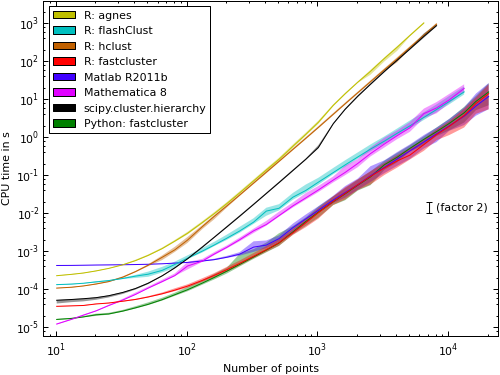
\includegraphics[scale=0.75]{images/FastComplete-CH3}
%\caption[Complete linkage clustering speed comparison between popular implementations.]{Different bands show maximum and minimum time over a variety of data sets. The average is plotted as a solid line. The synthetic data sets are samples drawn in an iid. manner from various mixtures of Gaussian distributions in Euclidean space of various dimensions.
%%The results were obtained on a PC with an Intel dual-core CPU T7500 with 2.2 GHz clock speed and 4GB of RAM. The operating system was Ubuntu 11.04 64-bit (Ubuntu 10.04 64-bit for Matlab R2010a). R version: 2.13.0, fastcluster version: 1.1.7, flashClust version: 1.01, Python version: 2.7.1, NumPy version 1.5.1, SciPy version: 0.8.0.
%(reprinted from \protect\cite{FastClust})}
%\label{fig:FastClustComparison}
%\end{figure}

I quickly linked up fastcluster to ES2, replacing our naive binning implementation and achieved impressive speed results (see Figure~\ref{fig:FastVsNaive} on page~\pageref{fig:FastVsNaive}).
\begin{figure}[h!]
\centering
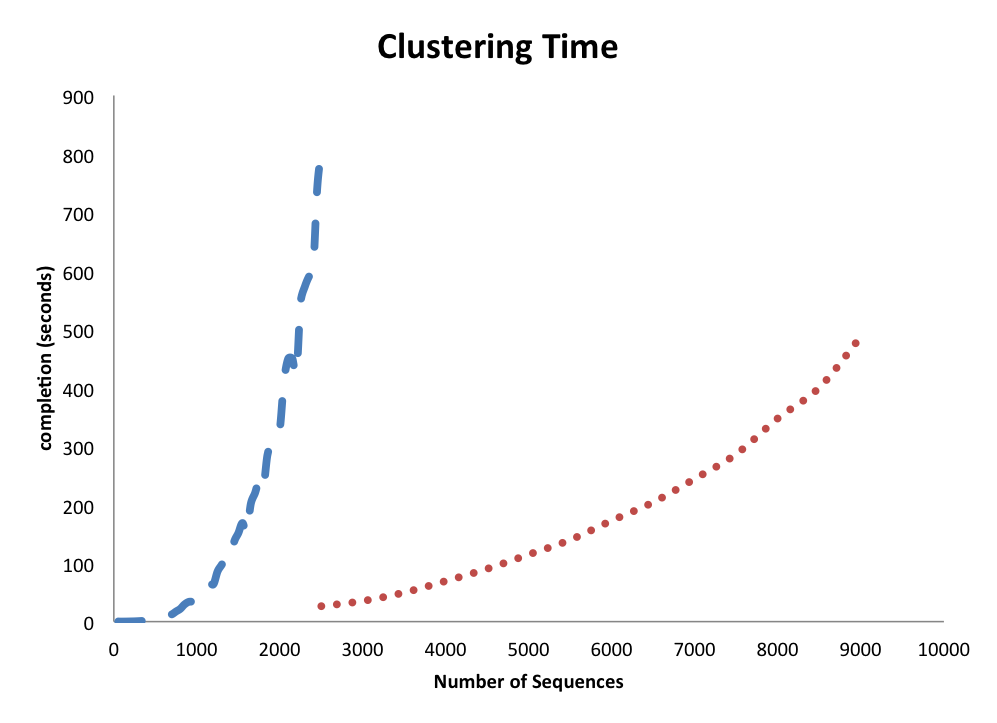
\includegraphics[scale=.8]{images/FastVsNaive-CH3}
\caption[Time comparison of fastcluster versus our naive implementation of complete-linkage clustering.]{Time comparison of fastcluster (dotted) versus our naive (dashed) implementation of complete-linkage clustering.}
\label{fig:FastVsNaive}
\end{figure}
Our current implementation was not capable of clustering datasets of greater than approximately three thousand sequences.
On the other hand fastcluster handled files with more than fifteen thousand sequences, until memory on my machine became a factor.
As far as accuracy goes, each bin level was within one or two of the current implementation (the slight error might be attributable to my quick hack job) in preliminary tests.
However, many more tests are needed to insure the package will work correctly for our purposes and we are not enthusiastic about adding another dependency to ES.
For now it is an envisioned improvement in the next version.

\subsubsection*{Minimizing space usage}
While increasing speed efficiency is important, the bottleneck has increasingly become space usage.
Our goal is to run ES on up to one million sequences, which in our current approach would entail a million squared pairwise distance matrix ($n \times n$).

In one exploratory approach we attempted to fix this problem by skipping the distance matrix generating step altogether.
Instead, we could define a replacement function that will calculate the distance between clusters at runtime (see Figure~\ref{code:LazyClustering} on page~\pageref{code:LazyClustering}).
\begin{figure}[h!]
\begin{algorithm}[H]
 \SetAlgoLined
% \KwData{c1 is a cluster of sequences, c2 is another cluster of sequences, seq-dist is a function that takes two sequences and returns the distance between them}
% \KwResult{the distance between two clusters}
\SetKwInOut{Input}{input}\SetKwInOut{Output}{output}

\Input{c1, c2 are different clusters of sequences}
\Output{The distance between two clusters, contained in $max$-$dist$}
\BlankLine
 $max$-$dist \gets 1.0$\\
 \For{$s1 \in c1$} {
   \For{$s2 \in c2$} {
    $d \gets seq$-$dist(s1, s2)$\\
    \If {$d < max$-$dist$} {
      $max$-$dist \gets d$
    }
   }
 }
\end{algorithm}
\caption[Pseudocode showing a distance function for two clusters.]{This pseudocode returns the distance between two clusters. The two clusters are represented by $c1$ and $c2$, while $s1$ and $s2$ represent sequences in the clusters. The function $seq$-$dist$ takes two sequences and returns the manhattan or taxicab distance between them.}
\label{code:LazyClustering}
\end{figure}
Clusters would start small, and then coalesce into larger clusters.
Thus the number of comparisons would remain relatively constant and there would be no distance matrix to store.
In this case, we would be choosing to minimize space usage, while greatly slowing down runtime.
It might be worth implementing a similar cluster distance function to use within the fastcluster complete-linkage implementation.
However, we would continue to hit a time limit easily.

%Approach two, bin in parallel.
A second option for minimizing space usage and runtime would be to develop (or find in the literature) a complete-linkage clustering algorithm that could run in parallel.
This strategy is still in early development.
The difficulty would be in splitting up the sequences into discrete tasks that could then be combined after computation.
Each of those discrete tasks could be spread out on a cluster, reducing run time, or even run at different times, freeing up memory.

Either way, there is much progress to be made at the binning step.
If ES is ever to work on one million sequences, the process of binning must be a major priority.

\subsection*{Demarcation}
The current automatic demarcation program has a serious problem with paraphyletic groups.
Instead of maintaining a species group when one of the organisms diverges, it forms many singleton groups, artificially inflating the number of ecotypes.
We believe this is part of the reason why if ES is run on a dataset with a low $npop$ value the output numbers become skewed.
As of yet, we are still unsure of ways to fix this problem.

Another issue with demarcation is speed.
We found that in many cases when we ran ES2 on large datasets the majority of time (\textasciitilde90\%) was spent demarcating~\cite{lingThesis}.
One potential solution would be to modify the demarcation confidence interval program so that instead of stepping down by $npop$ sequentially one at a time, determining likelihood, we could check the likelihood of $npop = 1$ from the start, thus more quickly deciding whether or not we are observing a single ecotype.
This approach is still quite experimental and I have not had a chance to test it.

\subsection*{Parallelization}
These days computer chips are not improving as dramatically as in the past.
Instead large computer clusters with thousands of nodes have emerged.
In the future we would like to access the power of computer clusters.

\subsubsection*{OpenMP approach}
The OpenMP API is a commonly used shared-memory parallelism approach designed for C, C++, and Fortran programs.
In Fortran the programmer adds comments (known as directives) to specify OpenMP behavior.
These directives implicitly or explicitly define or guide the execution of multiple threads as parallel programs.

An OpenMP enriched program begins as a single thread of execution.
Whenever a thread encounters a parallel construct the thread creates a team of sub-threads, generates a set of tasks, and then declares itself master of the team.
Only the master thread resumes execution beyond the end of the parallel construct.
The program can specify any number of parallel constructs.

All threads have access to the same memory so they can retrieve variables, this is called a shared-memory model.
Also, each thread can specify private memory unreachable to other threads.
We use shared and private clause keywords to identify the respective paradigm.

\subsubsection*{Tests}
%Outline best results from Ling's tests
\begin{figure}[h!]
\centering
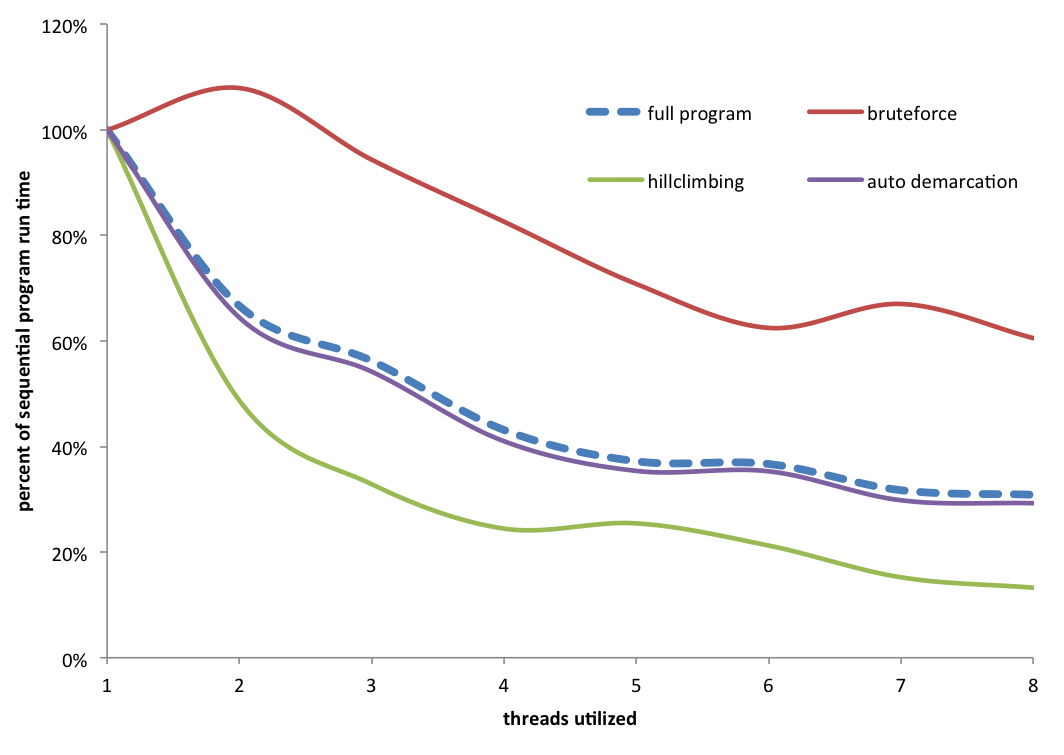
\includegraphics[scale=0.6]{images/LingParallelized-CH4}
\caption[OpenMP parallelization results.]{OpenMP parallelization results. Notice that the full program takes about half as much time when run with 8 threads. The full program run time follows the automatic demarcation program so closely because it took 90\% of the total run time in most cases (Figure adapted from \protect\cite{lingThesis}).}
\label{fig:LingParallelized}
\end{figure}

Lingyuan Ke ran the full ES2 program on Wesleyan computer cluster~\cite{lingThesis}.
It consists of 176 nodes, however we are limited to the shared-memory model parallelization so we can only use threads within a single node, thus up to 8 threads.
Figure~\ref{fig:LingParallelized} on page~\pageref{fig:LingParallelized} shows run times for all the programs as we increase the thread number.
The full program run time was decreased by half when we used 8 threads.
For more results on OpenMP parallelization refer to Lingyuan Ke's senior thesis~\cite{lingThesis}.

\subsubsection*{OpenMPI}
OpenMPI is an open source and complete message passing interface implementation of MPI-2 used in many of the world's largest computing clusters.
While OpenMP uses the shared-memory model, a message passing interface is used to run programs on mostly distributed memory systems.
It provides course grain parallelization across nodes as opposed to fine grain OpenMP parallelization within a processor~\cite{gabriel04:_open_mpi}.

We plan to capitalize on a hybrid OpenMPI-OpemMP paradigm to parallelize ES at the high level and low level.
At the high level we could divide the parameter search space over multiple nodes of the cluster, while at the low level, within each node, simulation replicates would be divided between the cores in the processor.
If correctly implemented ES could be run on clusters of almost any size, resulting in dramatic speed decreases.



\section{Finally}
%Might not need this section, then again some repetition might be good?
We have found that there are many areas to improve on in ES2.
This is an ongoing development process.
Parallelization using OpenMPI will lead to the greatest speed dividends in the near future.
However, an important emerging bottleneck is binning space usage.
We are considering, various approaches to the problem that include parallelization and algorithm switches.
Also, we have identified several issues with the automatic demarcation program leading to inflated $npop$ prediction in the presence of paraphyletic groups.
And as usual speed has become an issue for demarcation.
Even with these ideas for improvement we aim to release a production ready version of ES2 soon (it is already used for analysis in the Cohan lab).

Demarcation not limited by input size is an attractive goal, but we are not quite there yet.
We are continuing the Ecotype Simulation development in pursuit of bacterial species understanding that will eventually lead to practical applications.